\section{Deployment}\label{sec:03_depl}
% Explain section
This section explains the deployment of the application.
% Requirements
The requirements to run all applications are the following:
\begin{itemize}
\item H2
\item Wildfly
\item Java 11
\item Tomcat
\item Maven
\end{itemize}


% Create database
\subsection{Creating the Database}\label{sec:03_depl_createdb}
% What
As mentioned before, this application uses a local H2 database, that is not integrated in the project itself, but is located somewhere on the users computer.

% Create a Database
First, it is necessary to create a local database. Fig XY illustrates the process of creating a local database. First, it is necessary to change the directory to \path{H2_DIRECTORY/bin}. Then, execute the command \texttt{\$ java -cp h2-*.jar org.h2.tools.Shell}. It is important, that the databse is called \textit{accommodations}, and the username is \textit{sa}, and the the password is \textit{sa} as well.

% Start H2
After the database has been created, it is needed to start H2 via the terminal. To accomplish this, execute the command \texttt{\$ java -jar h2*.jar} in the directory \path{H2_DIRECTORY/bin}. This process is shown in \Fig{fig:03_depl_createdb_h2start}.
\begin{figure}[h]
\centering
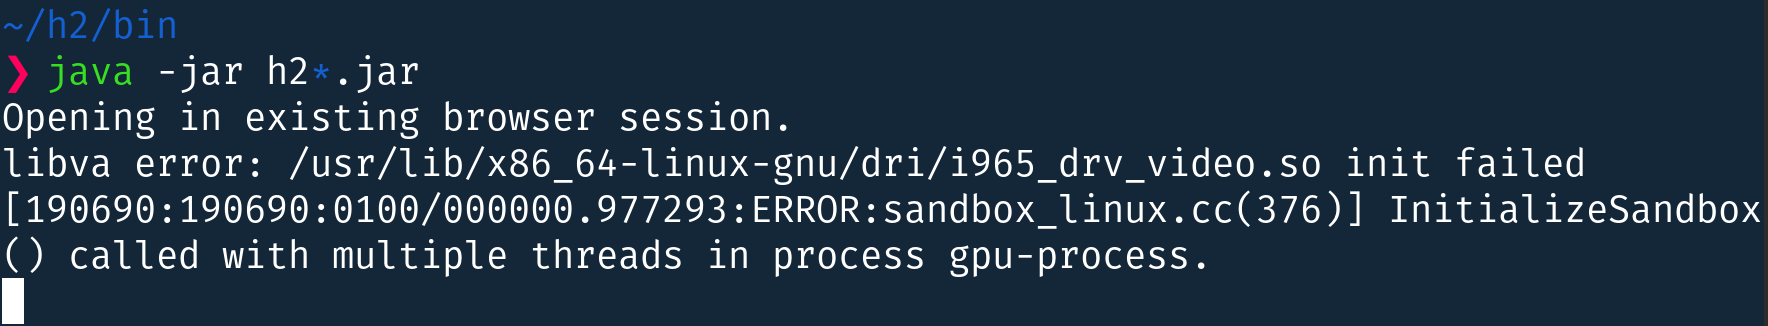
\includegraphics[scale=0.2]{images/03_depl/h2_start}
\caption{H2 database start process}
\label{fig:03_depl_createdb_h2start}
\end{figure}

% Web browser
After that, the web browser should open the H2 console automatically. At the H2 console, it is possible to test the database connection to see if the database has been created successfully.
% How to test
First, it is necessary to put in the correct JDBC URL in the format \texttt{jdbc:h2:tcp://localhost/PATH\_TO\_DATABASE/accommodations}. The username is \textit{sa}, and the password is \textit{sa} as well. After that, by clicking on \textit{Test Connection} it is possible to test the connection. \Fig{fig:03_depl_createdb_h2test} shows the message if the test was successful. After that, the database can be used in the application.
\begin{figure}[h]
\centering
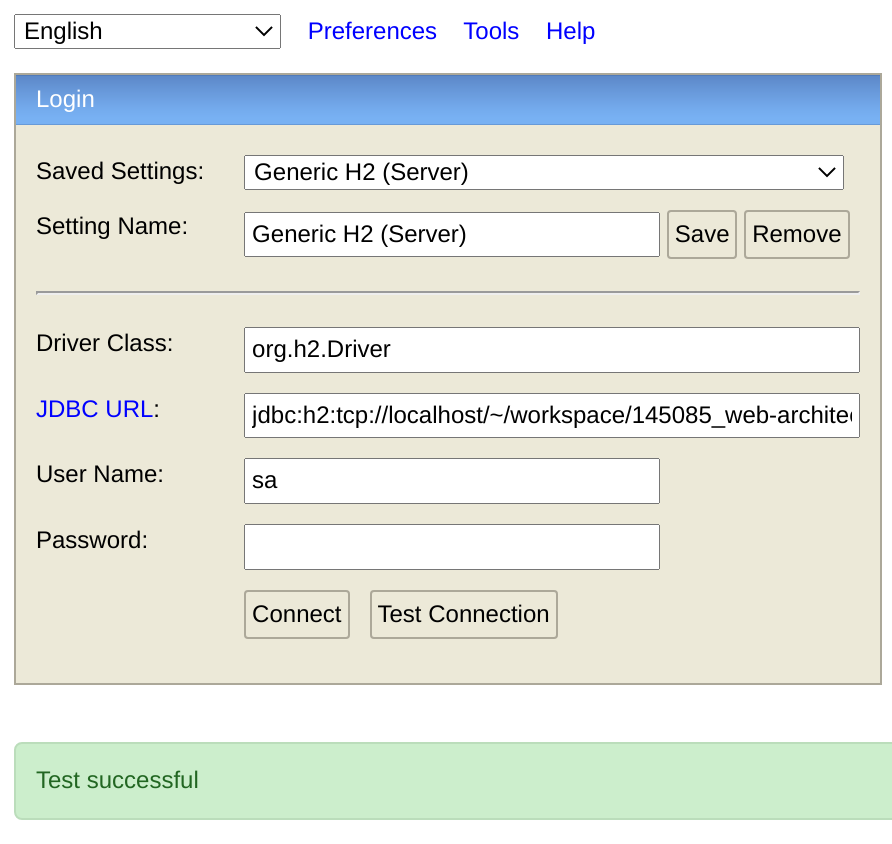
\includegraphics[scale=0.3]{images/03_depl/h2_test}
\caption{Successfull connection test for the H2 database}
\label{fig:03_depl_createdb_h2test}
\end{figure}


\subsection{Seeding the Database}\label{sec:03_depl_seeddb}
% What
After the database has been created, it is important to write dummy data to it using the \textit{DatabaseRoutine} application.

\subsubsection{Set up the DatabaseRoutine application}\label{sec:03_depl_seeddb_setup}
% How
It is important to set the path to the database in the \path{persistance.xml} of the \textit{DatabaseRoutine} application. \Lst{lst:03_depl_seeddb_setup_config} shows a correct configuration. The property \texttt{hibernate.connection.url} has to be set to the URL used in \Sec{sec:03_depl_createdb}.
\begin{lstlisting}[label=lst:03_depl_seeddb_setup_config, caption=Default data source configuration, language=xml]
...
<persistence-unit name="default">
  <properties>
    <property name="hibernate.connection.url"
              value="jdbc:h2:tcp://localhost/~/workspace/145085_web-architectures/assignment_5/accommodations"/>
  </properties>
</persistence-unit>
...
\end{lstlisting}

\subsubsection{Execute the DatabaseRoutine application}\label{sec:03_depl_seeddb_executeroutine}
% How
To execute the DatabaseRoutine application, open the project in IntelliJ, right-click on the DataRoutine.java file, and select \textit{Run 'DataRoutine.main()'}. Then, the file gets executes and write dummy data to the database.

% Check
After that, it is possible to check if the data has been written to the database by connecting to the database using the H2 console, introduced in \Sec{sec:03_depl_createdb}. FIG AB shows the newly created tables in the database.


\subsection{Setting up Wildfly}\label{sec:03_depl_wildfly}
% Set up Wildfly
At first, it is important to make sure, that Wildfly (mentioned in SEC AB) is available locally.

% Set up the datasource
\subsubsection{Add H2 database datasource}\label{sec:03_depl_wildfly_datasource}
Second, to access the database, the path to the previously created H2 database need to be set as a datasource in the configuration file of Wildfly. The configuration file is located at \path{WILDFLY_DIRECTORY/standalone/configuration/standalone.xml}. \Lst{lst:03_depl_wildfly_datasource_config} shows how the in \Sec{sec:03_depl_createdb} created H2 database can be added as a datasource in Wildfly.
\begin{lstlisting}[label=lst:03_depl_wildfly_datasource_config, caption=Default data source configuration, language=xml]
...
<subsystem xmlns="urn:jboss:domain:datasources:6.0">
  <datasources>
    <datasource jndi-name="java:jboss/datasources/AccommodationsDS" pool-name="AccommodationsDS" enabled="true" use-java-context="true" statistics-enabled="${wildfly.datasources.statistics-enabled:${wildfly.statistics-enabled:false}}">
      <connection-url>jdbc:h2:tcp://localhost/~/workspace/145085_web-architectures/assignment_5/accommodations;DB_CLOSE_DELAY=-1;DB_CLOSE_ON_EXIT=FALSE</connection-url>
      <driver>h2</driver>
      <security>
        <user-name>sa</user-name>
        <password>sa</password>
      </security>
    </datasource>
    ...
  </datasources>
</subsystem>
...
\end{lstlisting}

% Also to the project
Additionally, this datasource has to be defined in the \path{persistance.xml} configuration file of the WebServices project as well, which is shown in \Lst{lst:03_depl_wildfly_datasource_persistance}.

\begin{lstlisting}[label=lst:03_depl_wildfly_datasource_persistance, caption=Default data source configuration, language=xml]
...
<persistence-unit name="default">
  <jta-data-source>java:jboss/datasources/AccommodationsDS</jta-data-source>
  <properties>
    <property name="hibernate.show_sql" value="true"/>
    <property name="hibernate.format_sql" value="true"/>
    <property name="hibernate.use_sql_comments" value="true"/>
  </properties>
</persistence-unit>
...
%\end{lstlisting}


% Build EJB jar
\subsubsection{Compile EJB Jar}\label{sec:03_depl_wildfly_jar}
Third, the EJB`s need to to be deployed to the Wildfly server. Therefore, it is necessary to run the command \texttt{\$ mvn clean package} in the directory of the \textit{WebServices} project. After that, a new directory called \path{/target} was created in the root folder of the \textit{WebServices} project, where the EJB JAR \path{WebServices.1.0-SNAPSHOT.jar} is located, which is shown at \Fig{fig:03_depl_wildfly_jar_build}.
\begin{figure}[h]
\centering
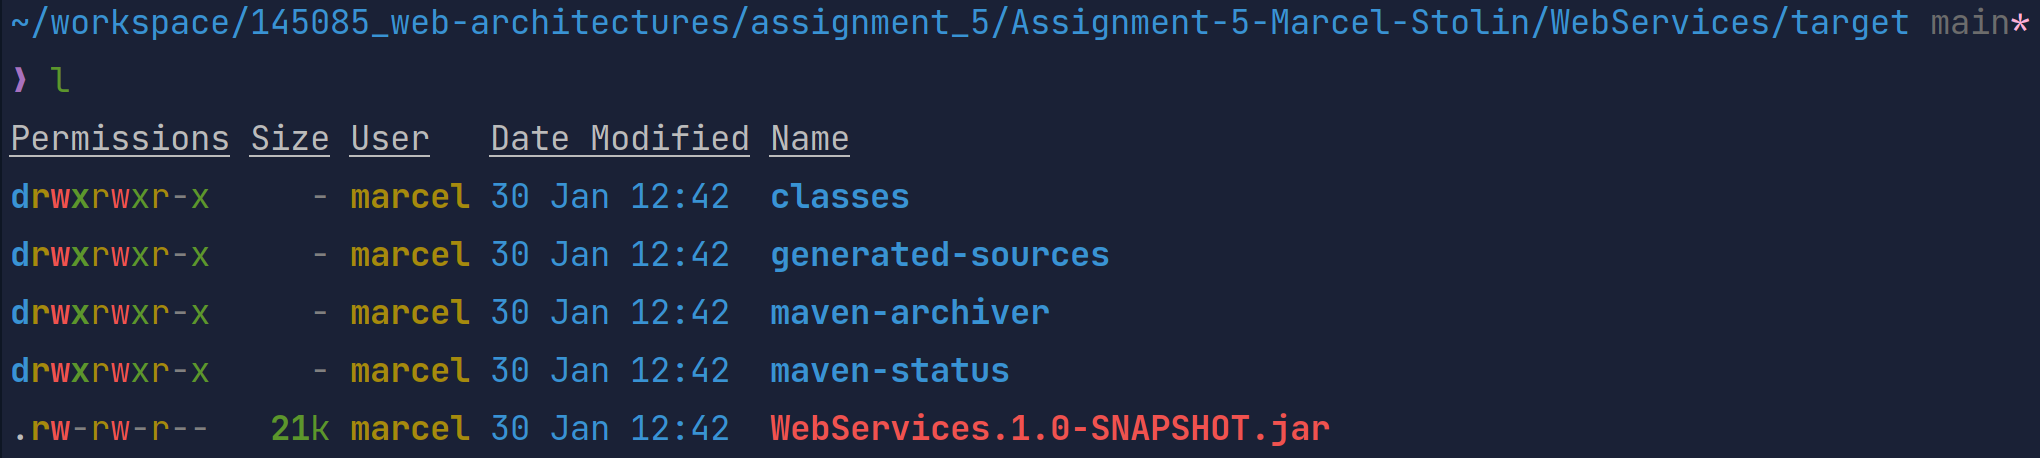
\includegraphics[scale=0.2]{images/03_depl/ejb-jar}
\caption{Successfull connection test for the H2 database}
\label{fig:03_depl_wildfly_jar_build}
\end{figure}


% Deploy jar
\subsubsection{EJB Jar Deployment}\label{sec:03_depl_wildfly_deploy}
After the \texttt{.jar} artifact has been created, it needs to be copied to the deployment directory of the Wildfly server. the deployment directory is located at \path{WILDFLY_DIRECTORY/standalone/deployments}. The artifact can be deployed using the command \texttt{\$ cp target/WebServices.1.0-SNAPSHOT.jar WILDFLY\_DIRECTORY/standalone/deployments}. This command needs to be executed in the project folder of the \textit{WebServices} project.


% Start Wildfly server
\subsubsection{Start Wildfly Application Server}\label{sec:03_depl_wildfly_start}
Finally, the Wildfly server can be started using the command \texttt{\$ bin/standalone.sh}. Additionally, the log shows the lookup address of both the \textit{AccommodationService} (mentioned in SEC XY) and the \textit{ReservationService} (mentioned in SEC AB), which is illustrated in \Fig{fig:03_depl_wildfly_start_addresses}.
\begin{figure}[h]
\centering
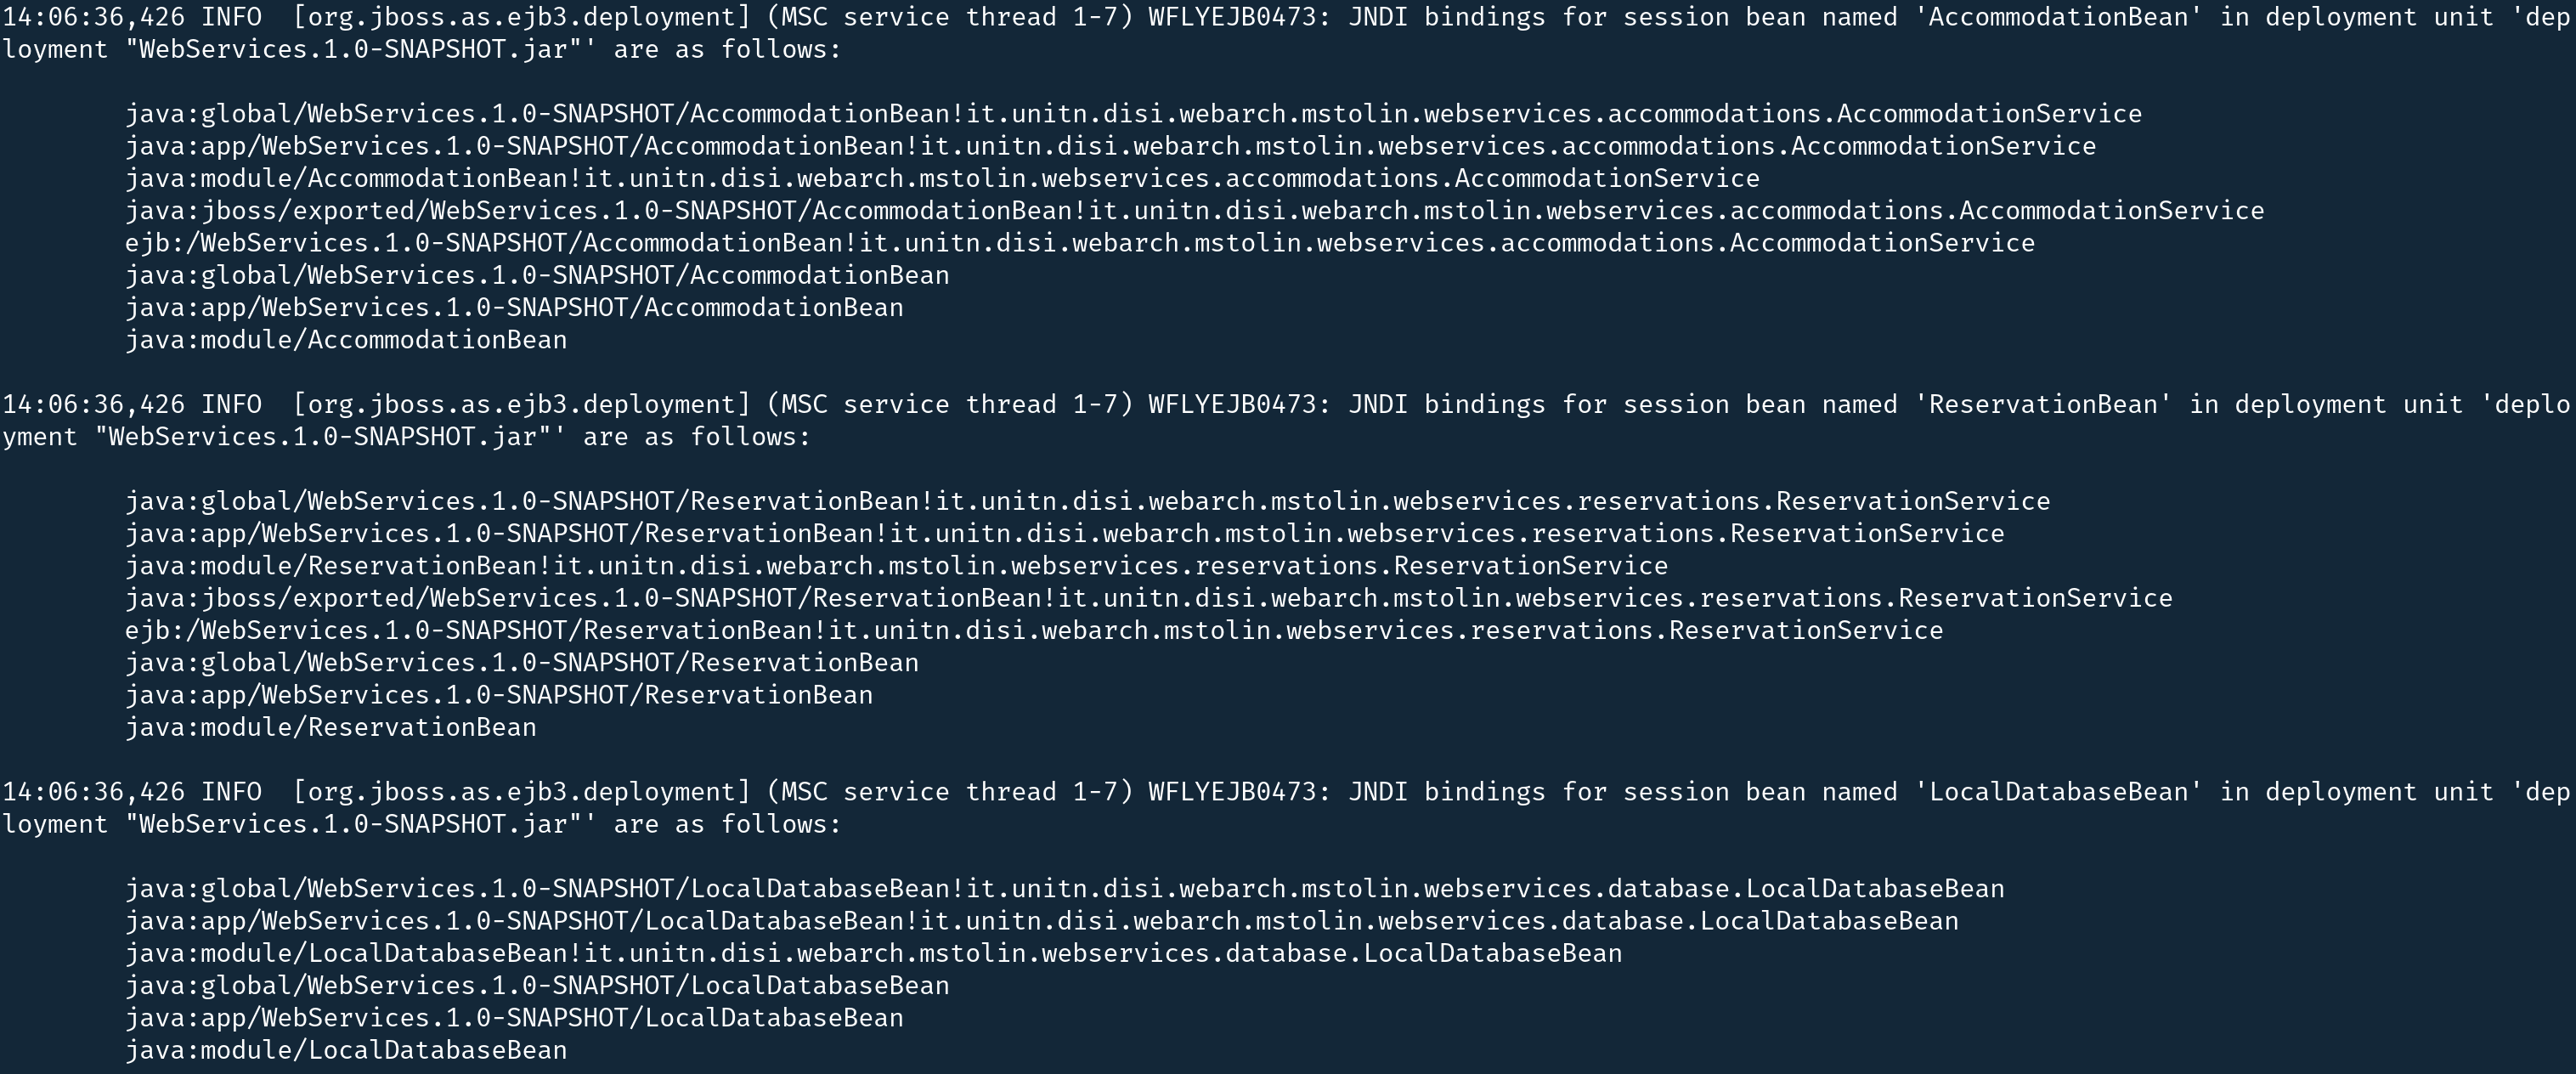
\includegraphics[scale=0.13]{images/03_depl/deployed_beans}
\caption{Successfull connection test for the H2 database}
\label{fig:03_depl_wildfly_start_addresses}
\end{figure}


\subsection{Starting the Web Application}\label{sec:03_depl_webapp}
% Important things
Before starting the web application it is important, that the following steps have been done in the given order:
% Steps
\begin{enumerate}
\item Start H2 database (\Sec{sec:03_depl_createdb})
\item Add data to H2 database (\Sec{sec:03_depl_createdb})
\item Set up H2 database as a Wildfly datasource (\Sec{sec:03_depl_createdb})
\item Compile and deploy EJB JAR artifact to Wildfly (\Sec{sec:03_depl_createdb})
\item Start Wildfly application server (\Sec{sec:03_depl_createdb})
\end{enumerate}

% Next
After those steps have been executed, the web application can be deployed and started using Tomcat.

% Create executable
\subsubsection{Build Artifact}\label{sec:03_depl_webapp_artifact}
First, it is necessary to create the \texttt{.war} artifact of the \textit{WebApp} project, using the command \texttt{\$ mvn clean package} which has to be executed in the \textit{WebApp} projects root directory. After that, a new directory called \texttt{target/} has been created which contains the artifact \texttt{marcel-stolin-web-app.war}.

% Deploy executable
\subsubsection{Deploy Artifact}\label{sec:03_depl_webapp_deploy}
After the artifact has been built, it needs to be deployed to the \path{webapps/} directory of the Apache Tomcat directory using the command \texttt{\$ cp target/marcel-stolin-web-app.war APACHE\_TOMCAT/webapps}.

% Set port
\subsubsection{Configure Port}\label{sec:03_depl_webapp_config}
One problem is, Apache Tomcat starts its service on port 8080 by default, which is also the default port of Wildfly. Therefore, the port of Apache Tomcat has to be changed to anaother port, e.g. 8000. The default port can be changed in the file \path{server.xml}, which can be seen in \Lst{lst:03_depl_webapp_config_server}.
\begin{lstlisting}[label=lst:03_depl_webapp_config_server, caption=Default data source configuration, language=xml]
...
<Service name="Catalina">
  <Connector port="8000" protocol="HTTP/1.1"
             connectionTimeout="20000"
             redirectPort="8443" />
</Service>
...
\end{lstlisting}

% Start server
\subsubsection{Start Server}\label{sec:03_depl_webapp_start}
Finally, the Apache Tomcat server can be started using the command \texttt{\$ APACHE\_TOMCAT/bin/catalina.sh start}. After that, the web application is available at \url{http://localhost:8000/marcel-stolin-web-app/}, as shown in FIG XY.
